\documentclass[a4paper,12pt]{article}
\usepackage{t1enc}
\usepackage[longnamesfirst, round]{natbib}  % Bindet den natbib-standard fuer das Zitieren ein
\usepackage{epsfig}
\usepackage[latin1]{inputenc}   % Ermoeglicht Sonderzeichen direkt einzugeben
\usepackage[T1]{fontenc}        % Garantiert saubere Worttrennung bei Umlauten etc.
\usepackage{color}              % Farbpaket
\usepackage{amsmath,amsfonts,amssymb}   % ermoeglicht mathematische Sonderzeichen
\usepackage{ngerman}           % neue deutsche Rechtschreibung
\usepackage[english]{babel}     %
\usepackage{ae}                 %
\usepackage{graphicx}           % Ermoeglicht das Einbinden von Bildern in allen Formaten
\usepackage{longtable}          % zum erstellen von Tabellen ber mehrere Seiten
\usepackage{multirow}           % zum Verbinden von Zeilen innerhalb einer Tabelle
\usepackage{booktabs}			% für tablegenerator 
%\usepackage{pictexwd}           % PicTex, ein Graphikpaket
%\usepackage{pst-all, multido}   % psTricks, ein Graphikpaket
\usepackage{url}



% ________________ EINRICHTEN DES DOKUMENTS ______________________%

\bibliographystyle{plainnat}    % legt den Stil fuer das Inhaltsverzeichnis fest

\oddsidemargin 0.1in \evensidemargin 0.1in \textwidth 15.5cm \topmargin -0.4in \textheight 24.5cm
\parindent 0cm      % legt die Seitenraender fest

\pagestyle{plain}          % leere Kopfzeile, Seitennummer in der Mitte der Fusszeile

\newcommand{\bs}{\boldsymbol}  % shortcut zur Erzeugung von fetten Sympolen in der Mathe-Umgebung

\renewcommand{\baselinestretch}{1.25}
% 1,5 -facher Zeilenabstand (Standard ist 1,2-facher Zeilenabstand, also 1,2*1,25 = 1,5



\begin{document}

% ________________ TITELSEITE ______________________%


\pagenumbering{roman}   % roemische Zahlen zur Seitennumerierung

\begin{titlepage}       % Umgebung fuer Titelseite, frei gestaltbar

\thispagestyle{empty}   % keine Numerierung auf Titelseite


\begin{center}
\vspace*{2.5cm}
{\bf  \Large The Distribution of Wealth \\in a Life-Cycle Model with Durables} \\
\vspace*{3cm} 
Master Thesis \\ in Economics \\
Prof. Dr. Thomas Hintermaier  \\
\vspace*{0.5cm} 
Summer Term 2017\\
\end{center}

\vfill
\begin{flushright}
   \emph{Eric Lustenberger} \\
    \emph{Heckenweg 38}\\
    \emph{3007 Bern}\\
   \emph{Student Number}\\
 \emph{Economics}\\

\end{flushright}



% 
% \begin{center}
% $ $			% oeffnet und schliesst eine Matheumgebung (Trick, um den Titel nach unten zu rutschen
% \vspace{4cm}
% 
% {\LARGE TITEL}
% \vskip 4cm
% 
% Diese Seite ist frei gestaltbar
% \end{center}

\end{titlepage}

\newpage                % erzwingt an dieser Stelle einen Seitenumbruch



% ________________ INHALTSVERZEICHNIS ______________________%


% \tableofcontents   %fuegt Automatisch ein Inhaltsverzeichnis ein
% 
% \newpage
% 


% ________________ HAUPTTEIL ______________________%


\pagenumbering{arabic}      % Seitenzahlen wieder arabisch numerieren
\setcounter{page}{1}        % Ruecksetzen des Seitenzahlzaehlers auf 1


\section{Introduction}
\label{Chapter1}

The main goal of this paper is to show how modeling durables in an incomplete markets life-cycle model where agents face idiosyncratic income shocks and thus accumulate precautionary savings can help to explain how agents accumulate wealth over the life-cycle. Such models provide the basis for the analysis of redistributional policies. They shed light on the underlying mechanisms leading to unequal distributions of wealth and consumption. In order to improve policy making it is crucial in understanding these mechanisms. 

My starting point is a classical life-cycle model with incomplete markets such as \cite{hintermaier2011} use. A majority of the literature focuses on models with only one asset, net worth. However, as \cite{FV&K2011} show, modeling durables has a big impact on life-cycle savings. Others such as \cite{diaz2010} show how modelling durables affect the wealth distribution. My thesis contributes to this literature and shows that modeling durables (is either important or unimportant) in order to reproduce the wealth distribution. And thus sheds light on the importance of durables as important driver of the net-worth accumulation. 

\section{Literature Overview}
\label{Chapter2}

THIS SECTION WILL BE SPLIT UP INTO INTRODUCTION, FACTS AND GENERATING A WEALTH DISTRIBUTION

Investigate empirical predictions of the life-cycle incomplete markets model (\cite{Gourinchas&Parker2002}; \cite{cagetti2003}; \cite{castaneda2003}; \cite{yang2009}; \cite{kaplan2010}; \cite{hintermaier2011}), thus contribute to the literature that (note copy paste.... demonstrate that a plausibly parameterized version of their models can quantitatively explain empirical findings as arising from rational choices of consumers facing an increasing wage profile and income uncertainty.)
The model is based on the classic income-fluctuation problem in which the consumer faces a stochastic income process and decides in every period how much to save and how much to consume. Important contributions to the literature are Deaton (1991), Carroll (1992,1997), \cite{Gourinchas&Parker2002}. (note copy paste... Following Bewley (1986), this problem has been embedded by Huggett (1993) and Aiyagari (1994) into a general equilibrium framework, giving rise to the endogenous determination of the interest rate as well as a nontrivial income, wealth, and consumption distribution at equilibrium.)
(Note copy paste... Furthermore, this paper relates to other literature such as: 
Endogenous borrowing constraint: The specification of the borrowing constraint  in \cite{FV&K2011} is adapted from the recent endogenous incomplete-markets literature: Kehoe and Levine (1993), Kocherlakota (1996), Krueger and Perri (1999, 2006), and Alvarez and Jermann (2000). Lustig (2004) also has a model with durable assets and an endogenous borrowing constraint to explain the equity premium puzzle, however agents have full access to Arrow securities and are infinitely lived.
Literature on optimal portfolio choice in the presence of consumer durables: Grossman and Laroque (1990), Eberly (1994), Chah et al. (1995), and Flavin and Yamashita (2002).)

Note: missing citations, not all of the above are cited properly!!!!!

Literature on wealth distribution!!!!! 

\section{Facts about the wealth distribution}

\section{Generating a wealth distribution}
\label{Chapter3}
In the following section I discuss the economic model considered and outline the most important considerations made within the literature. Firstly, I discuss the life-cycle modeling and the literature, which applies life-cycle and to be more exact imperfect markets models in the context of wealth distributions. Secondly, I present my modeling choices and solution methods applied for this particular problem. 
\subsection{Modeling Literature}

\subsection{The Model}
Before going into a more detailed description of the model at hand it is important to understand the modelling choice. Why a life-cycle model with an imperfect market structure? Why include durables as an  additional asset choice to the more standard approach, which does summarize all assets in a one period bond, such as for example \cite{hintermaier2011}? 

To answer the first question I will mainly refer to the the literature. The second will be discussed in a more detailed manner in the following section, which treads the life-cycle profiles and especially the importance of modeling durables. 

\subsubsection{Imperfect market structure}
The choice of an exogenously determined imperfect market structure allows for a straight forward answer. It comes down to the economic question one poses. The aim here is to demonstrate that such a model can quantitatively explain the empirical net-wealth distribution in the US. The role the imperfect market structure, entering as a limited choice of assets to fully insure against idiosyncratic wage shocks, poses, is thus to produce an endogenous wealth distribution. The savings are fist and foremost driven by a precautionary motive to insure for future wage shocks. Knowing that the income may drop in the future consumers save today to achieve a more stable consumption across their live. In a complete market framework consumers could perfectly diversify away idiosyncratic risks \citep{a&w2010}  (and thus would not build a buffer stock of savings for future shocks.) (???????? is this exact?????)
The hypothesis of the complete market framework has been rejected by the vast majority of empirical research \citep{a&w2010}. \cite{deaton1994} show that the life cycle profile of consumption inequality is increasing with age, a fact that would be inconsistent with complete markets. Moreover, the assuming away markets, where individuals can trade contingent claims to insure themselfs against the idiosyncratic wage shocks is justified by moral hazard problems \citep{FV&K2011}. While in some rare cases - such as when only studying aggregates, it may still be sufficient to consider a complete market framework, when considering wealth-distributive questions, the imperfect market assumption is both necessary from a theoretical perspective and well-founded from an empirical perspective. It remains to discuss the whether it makes sens to treat distributive issues from a life-cycle point of view.

\subsubsection{Life-Cycle}

As \cite{deaton1994} show, consumption inequality seems to vary with age. Further empirical research does support these findings, indicating that some of the differences in earnings, income, and wealth across households can be attributed to differences in the household's age \cite{rios2016} (FIND BETTER REFERENCES?). \cite{hintermaier2011} Show that the average net-wealth increases with wealth and that the dispersion of wealth falls with age. 
Moreover, there is a vast theoretical literature using a different versions of the life-cycle model to discuss distributive questions.  \cite{Gourinchas&Parker2002}; \cite{cagetti2003}; \cite{castaneda2003}; \cite{yang2009}; \cite{kaplan2010};\cite{hintermaier2011} (CITE MORE RECENT LITERATURE!!!)
while there are also some that use infinite horizon models....

Finally, the choice to study the empirical validity of a life-cycle model, which produces a net-wealth distribution arising from rational choices of consumers subject to income uncertainty, moreover allows for a detailed analysis of consumption and savings behavior over a person's live-cycle. A coherent framework incorporating the behavior of household's over their lifespan is paramount for the study of re-distributive policies. (Cite....)
These factors thus support the choice of a life-cycle model. 


\subsubsection{Partial Equilibrium}
Last but not least, partial equilibrium as modeling choice has to be discussed briefly. (????????????????)

(copy paste from hintermaier 2011
Note that we assume that changes in the domestic supply of assets do not affect do not affect the interest rate. As in a small-open economy, this price is determined exogenously (on the world markets.) \footnote{This assumption is not restrictive for our purposes since we observe the price in our ex post analysis for the period 1983-2007. Hence, the supply of assets and the observed price suffice to determine the equilibrium asset quantities. This allows us to be agnostic about the price elasticity of asset demand.})

\subsubsection{The Income Process}
\cite{kaplan2010} discuss various features of the income process in more detail.


\subsubsection{Consumer's Problem}
As established above, the baseline model in question is a life-cycle model with an imperfect market structure. I closely follow \cite{hintermaier2010}.\footnote{In order to facilitate comparability, I will closely follow the notation used in their paper.} While there algorithm allows for both a live-cycle and infinite-horizon models, the example model presented in their paper uses the latter. For reasons discussed above, I will in this case opt for a live-cycle formulation. Finally, the baseline model does not include adjustment costs. These are considered in a later section of the model. 

There is a continuum of risk averse consumers with a finite time horizon. 
At age 90 consumers die with certainty, younger consumers between the age of 26 and 90 may die with probability $\pi_{j} < 1$ at age $j$. Until retirement the labor income of each individual $i$ $y_{ij}$ is stochastic. After the age 65 is completed, they retire with certainty and receive individual-specific retirement benefits $b_{i}$.\footnote{The construction of these benefits is discussed in the Appendix.}
Consumers derive utility from a durable good $d$ and a non-durable good $c$. The utility function $U(c,d)$ is strictly concave, increasing and non-separable in c and d (REALLY??? When not??? all three true???). 
In each period consumption $c_{j}$, the durable good $d_{j+1}$ and the financial risk-free asset $a_{j+1}$ are chosen after receiving the income. Agents then derive utility from consumption and durable services, before the assets pay returns. While the liquid assets return an interest rate $r$ durables depreciate at rate $delta$. As previously discussed, such a market structure implies that markets are incomplete and agents will accumulate a buffer stock in order to save for rainy days. The ex-ante identical consumers thus will thus, depending on their income trajectory, end up with different portfolios of the endogenous state variables. The model is therefore suited to match empirical facts about net worth positions since it does produce an endogenous distribution of portfolios, which differs in age and income. Moreover, (THE ADVANTAGE OF DURABLES) besides providing services and thus allowing consumers to derive utility from durables, their durability implies, that they may be used as collateral. It is assumed that all credit needs to be collateralized.\footnote{About 85\% of household debt in the Survey of Consumer Finances 2004 is secured by collateral.\citep{hintermaier2010}} 
\\
The collateral constraint takes the form:

\begin{equation}
\underbrace{\mu(1-\delta)d_{j+1} + \gamma\underline{y}}_{collateral} \geq -(1+r)a_{j+1}
\end{equation}

where $\underline{y}$ is the minimum labor income realization \footnote{CHECK THIS WITH CODE!!!} and $\mu \in [0,1) and \gamma \in [0,1)$ are the respective fractions of the durable stock and of minimum labor income, which can be collateralized.
\footnote{It is important to note that this constraint guarantees full repayment by consumers and thus acts as non-bankruptcy constraint. This is assured by the timing assumptions made above \textendash The lender does know the financial portfolio choice $(a_{j+1},d_{j+1})$ and the minimum of the support of the income distribution $\underline{y}$, however future individual income draws $y_{j+1}$ do remain obscure to him. Finally, note that only choices in $j$ determine, whether the constraint is binding or not. }

It is useful to rewrite the constraint in terms of total wealth and future durable holdings. Total wealth available to a consumer in each period is 

\begin{equation}
x_{j} \equiv (1+r)a_{j} + (1-\delta)d_{j},
\end{equation}

rewritten the constraint then looks like this:

\begin{equation}
x_{j+1} \geq -\gamma\underline{y}+(1-\mu)(1-\delta)d_{j+1}
\end{equation}

One now sees that total wealth needs to be larger than the negative value of the minimum fraction of income that can be collateralized and the fraction of wealth which cannot be used as collateral. Furthermore, under the assumption that $\mu < 1$ $d_{j+1}$ is determined for a given $x_{j+1}$, when the constraint binds.

Although in my baseline model they are set to 0, I also consider the case where durables can only be adjusted with some costs: 

\begin{equation}
\Psi(d_{t+1},d_{t})=\frac{\alpha}{2}\left(\frac{d_{t+1}-(1-\delta)d_{t}}{d_{t}}\right)^2d_{t}.
\end{equation}\footnote{\citep{hintermaier2010} use the same specification, which is based on the investment literature (COPY PASTE(see, for example, \cite{adda2003dynamics},p.192)). Costs are differntiable in $d_{t+1}$ and $d_{t}$. Moreover, by letting the durable stock depreciate, consumers can avoid these costs. In this particular specification, adjustment costs do not affect the collateral constraint, as it is assumed that these costs do not have an impact on the sales of collateral seized by lenders. NOTE \citep{hintermaier2010} EXPLAIN IN APPENDIX VERSION WHERE THIS IS THE CASE.}

Finally, the specification of the budget constraint, follows from the above:

\begin{equation}
a_{j+1}+d_{j+1}+c_{j}+\Psi(d_{t+1},d_{t})=x_{j}+y_{j}
\end{equation}



\paragraph{The recursive formulation of the household problem} 

I will proceed by depicting the case prior to retirement. (SPECIFY RETIREMENT CASE!!!)
We let $T^{r}$ denote the first period of retirement.
The Bellman equation prior to retirement, if  $j < T^{r}$thus is:

\begin{equation}
v_{j}(x_{j},d_{j},y_{j}) = \max_{\substack{a_{j+1},d_{j+1}}}\left[U(\underbrace{x_{j}+y_{j}-a_{j+1}-d_{j+1}-\Psi(d_{t+1},d_{t})}_{c_{j}},d_{j})+\hat{v_{j}}(x_{j+1},d_{j+1},y_{j})\right]
\end{equation}

where the expected next period value function is discouted by the product of the probability of survival $(1-\pi_{j})$ and the discount factor $\beta$
\begin{equation}
\hat{v_{j}}(x_{j+1},d_{j+1},y_{j}) \equiv \beta (1-\pi_{j})E_{j}v_{j+1}(x_{j+1},d_{j+1},y_{j+1}),\textnormal{\footnote{Note that the income $y_{j}$ ensters the expected value of next period's utility function as a state, due to its persistence.}}
\end{equation}



with the constraints: 

\begin{equation}
a_{j+1}+d_{j+1}+c_{j}+\Psi(d_{t+1},d_{t})=x_{j}+y_{j},
\end{equation}

\begin{equation}
x_{j+1} = (1+r)a_{j+1} + (1-\delta)d_{j+1},
\end{equation}

\begin{equation}
x_{j+1} \geq -\gamma\underline{y}+(1-\mu)(1-\delta)d_{j+1}, 
\end{equation} (WHAT HAPPENS WITH MIN Y IN RETIREMENT????)

\begin{equation}
d_{j+1} \geq d_{min},
\end{equation}


FROM RED PAPER HELP TO SPECIFY CASE WITH RETIREMENT!!!
We specify our model in discrete time. Rearranging the budget constraint, consumption of individual $i$ with age $j$ is 

\begin{equation}
c_{ij} = 
  \begin{cases}
    (1+r)a_{i,j-1}-a_{ij}+y_{ij} & \quad \text{if } j < T^{r}, \\
    (1+r)a_{i,j-1}-a_{ij}+b(z_{i,T^{r}-1}) & \quad \text{if } j \geq T^{r},\\
  \end{cases}
\end{equation}

where $b(z_{i,T^{r}-1})$ are the retirement benefits. These benefits depend on the last realization of labor income before retirement $z_{i,T^{r}-1}$ as we explain further in the next section. Defining cash-on-hand as 

\begin{equation}
x_{ij} = 
  \begin{cases}
    (1+r)a_{i,j-1}+y_{ij} & \quad \text{if } j < T^{r}, \\
    (1+r)a_{i,j-1}+b(z_{i,T^{r}-1}) & \quad \text{if } j \geq T^{r},\\
  \end{cases}
\end{equation}

we can write the Bellman equation as 

\begin{equation}
V_{j}(x_{ij},y_{ij})= \max_{ \substack{a_{ij} \geq 0}}[u(\underbrace{x_{ij}-a_{ij}}_{c_{ij}}) + \beta(1-\delta_{j})E_{j}V_{j+1}(x_{i,j+1},y_{i,j+1})],
\end{equation}

where we restrict the choice of assets to $a_{ij} \geq 0$, as motivated in the previous section.)

\subsubsection{Numerical algorithm}

The problem above does not provide a closed-form solution and thus the solution has to be approximated numerically. As already mentioned above, the model is based on \cite{hintermaier2010} and I can therefore directly apply their algorithm. They expand the endogenous gridpoints method (EGM) proposed by \cite{carroll2006} for a problem with two states and thus providing a very efficient algorithm to solve models with durables and collateralized debt. \footnote{Solving such models has been considered particluarly expensive and challenging, as durables enter as additional state (if non-separability utility from durables and non-durable or adjustemnt costs are allowed for) and durables increase the dimensionality of the portfolio choice.\citep{hintermaier2010}} 

(NOTE THAT ALGORITHM MUST BE CHANGED FOR CASE WITH ADJUSTMENT COSTS)

Given the life-time sequences for income (as described in the income process section) {$y_{kj}$} and survival probabilities (CHECK ON HOW TO BEST WRITE DOWN!) {$(1-\pi_{j})$}, $\forall j = 1,...,T $ (AND ALL MARKOV STATES $k$) the algorithm starts with an exogenous grid for the future state $x', G_{x'} \equiv {x'_{1},x'_{2},...,x'_{I}}$, the current state $d, G_{d} \equiv {d_{1},d_{2},...,d_{J}}$.

The algorithm starts iterates recursively over the policy function starting with the last period $j=T$ in which the consumer sells all durables and liquid assets to consume before death. It thus holds that $x'=d'=a'=0$ and thus the initial consumption policy is $c(x,d_{j},y_{kj})=x+y_{j,k}$.For each period t < T-1, the algorithm proceeds as follows. In a first step it maps $x'$ into $d'$ and in a second step it solves for the current choice c and state x from optimal future combinations (x',d'). Moreover, the values for the exogenous grid are chosen such that the results are not affected. (BE MORE PRECISE
INDICATE DIFFERENCES BETWEEN POST/PRE RETIREMENT (expectation)!




NOT NECESSARY FROM HERE ON. HOWEVER MAYBE BE MORE PRECISE ABOVE!


For each period t < T-1, the algorithm proceeds as follows: 

\paragraph{Step 1: Mapping $x'$ into $d'$} 

Using the optimal relationship,
\begin{equation} \label{eq:optimal_algorithm}
\tiny
K_{ijk}\left((1+r)\left(1+\frac{\partial \Psi(d'_{ijk},d_{j})}{\partial d'}\right)-\mu(1-\delta)\right)-\eta_{ijk} = -\left(\frac{\partial \Psi(d'_{ijk},d_{j})}{\partial d'}(1+r)+r+\delta \right) \frac{\partial \hat{v}(x'_{i},d'_{ijk},y_{k})}{\partial x'}+\frac{\partial \hat{v}(x'_{i},d'_{ijk},y_{k})}{\partial d'},
\end{equation}
in the algorithm determines the values of, $d'_{ijk}$ for a given $y_{k}$ and $d_{j}$, which correspond to each of the exogenous gridpoints $x'_{i}$.\footnote{The partial derivatives are obtained by exploiting the envelope conditions. When considering adjustment costs one therefore has to solve for $\partial \Psi(d'',d') /\partial d'$. In the first iteration this is done by making use of terminal condition $d''=0$. For every iteration that follows $d''$ is then replaced by the previously computed optimal policy.(COPY PASTE: Note that with adjustment costs, full decumulation is feasible for all x,d and y if $\mu < 1-(1-\delta)\alpha/2$, which is satisfied for the chosen parameters below!!!!!!!!!!!}

There are three possible cases for each  $y_{k}$ and $d_{j}$, to compute the optimal $d'_{ijk}$.\footnote{Note that the optimal solution necessarily lies in the interval imposed by the collateral constraint and the lower bound on $d'$, $[d_{min},\bar{d_{i}}]$, where $\bar{d_{i}} \equiv \frac{x'_{i}+\gamma \underline{y}}{(1-\mu)(1-\delta}$.}
\paragraph{Case 1 \textendash  Neither the collateral nor the constraint on durables are binding} Hence, $K_{ijk}=\eta_{ijk}=0$ and thus the there exists a $d'_{ijk}$ for which the right hand side of \ref{eq:optimal_algorithm} is 0.
\paragraph{Case 2 \textendash the right hand side of \ref{eq:optimal_algorithm} is positive} jklh
\paragraph{Case 3 \textendash the right hand side of \ref{eq:optimal_algorithm} is negative} lkjg

\paragraph{Step:2 Obtaining current choice c and state x from optimal future combinations (x',d')}

\subsubsection{Comparing the simulation output with SCF data}

\subsubsection{Calibration}

\paragraph{Utility Function}
I consider the same class of preferences as \cite{hintermaier2010}, which is commonly used in the literature considering durable and non-durable consumption (CITE MORE). 

\begin{equation}
U(c,d)=\frac{\psi(c,d)^{1-\sigma}-1}{1-\sigma} \ \ \textnormal{where} \ \ \psi(c,d)=c^{\theta}(d+\epsilon_{d})^{1-\theta}, \ \textnormal{\footnote{The Cobb-Douglas specification is approximately validated by empirical evidence \citep{FV&K2011}}}
\end{equation}

where I assume $\epsilon_{d} > 0$, which thus indicates a number small enough to be irrelevant for the quantitative exercise at hand but nonetheless larger than zero. The utility function thus allows for zero consumption of durables, while the INADA-Condition ensures that people always consume some non-durables, i.e. they cannot survive without food, but are allowed to survive without houses and cars.(NOTE MIGHT LOOK AT DIFFERENCE BETWEEN EQUAL TO ZERO AND NOT EQUAL TO ZERO SINCE HINTERMAIER ALLOWS FOR BOTH(COPY PASTE: Allowing for the potentially optimal choice $d' = d_{min}$ means that the constraint for minimal durable holdings needs to be taken into account in the recursive problem as another occasionally binding constraint in addition to the collateral constraint!!!). 

The utility function thus, is strictly increasing durable consumption and non-durable consumption, strictly concave and obeying the Inada conditions with respect to nondurable consumption. 

\citep{FV&K2011} utility form death is normalized to 0 ??????????

\paragraph{Data (Initializing DATA + probability of death (PLOT!)}

\paragraph{Income Process}

LOOK AT GOURINCHASandPARKER(2002) AND AT THE ADDAandCOOPER BOOK! 

\begin{enumerate}
\item \citep{FV&K2011} stochastic labor income process up to age 65, where they impose mandatory retirement. Differs from other specifications such as Abowd and Card (1989), Carroll (1992), or Gourinchas and Parker (2002) in two aspects: 
\begin{enumerate}
\item do not allow labor income to go to zero- very low probability Carroll (1992) estimates it at 0.003 for a year. However, its effects on the intertemporal allocations are quite big, since hh will not borrow any positive amount since they might face a lifelong sequence of zero labor income and might be unable to consume a positive amount and repay their debt in some period. (Moreover, argument of public income-support programs in the US -> labor in the model is after-tax, after-government transfer labor income.
\item unit root in AR process is not imposed  ( is something that is debated -> they show that their results are not very sensitive toward this issue -> increase $\rho$ toward unity (LOOK AT STORESLETTEN ET AL: (2001) -> do not reject unit root.
\end{enumerate} 
\item Check \cite{hintermaier2010} and \cite{hintermaier2011}
\end{enumerate}

\paragraph{Others NOTE: INCOMPLETE LOOK AT PAPERS}
\begin{enumerate}
\item The interest rate
\begin{enumerate}
\item \citep{FV&K2011} $r = 4\%$(NOTE CITING A WORKING PAPER!!!) \footnote{\citep{mcgrattan2001}}

\item \citep{hintermaier2010} (COPY PASTE: The annual real interest rate is set to 3\% and the depreciation rate is 2\% (see, for example, Caporale and Grier, 2000; Lustig and van Nieuwerburgh, 2005). The low depreciation rate is motivated by the dominating role of housing for consumer durables.
\end{enumerate}
\end{enumerate}

\begin{enumerate}
\item Preference Parameters
\begin{enumerate}
\item  \citep{FV&K2011} $\theta = 0.81$ and $\beta = 0.9375$ matching the ratio of expenditures on nondurables and durables $C/I^{d} = (C/Y)/(I^{d}/Y) = 6.2$, which is the long-run average for U.S. data.

\item \cite{hintermaier2010} choose $\sigma = 0$, commonly used in the literature and then calibrate $\theta$ and $\beta$ to match (up to precision $10^{-2}$) the amount of wealth in total data, 6.33 in terms of average population labor earnings taken after taxes and transfers, and the part of wealth accounted for by durables, 4.45. \footnote{When they compute the statistic in the data, they use sampling weights provided in the SCF. (COPY PASTE: Note that the normalization by net labor and the use of equivalence scales implies that normalized (aggregate) wealth is larger than the wealth to output ratio.)}
\end{enumerate}
\end{enumerate}
\section{Why model durables? How do durables affect savings?}
\begin{enumerate}
\item \cite{FV&K2011} 
\begin{enumerate}
\item empirical observation that durables constitute a large fraction of households' asset holdings - hh hold 35\% of their total assets in durables and only 28\% in equity (flow of funds account 2nd quarter) 
\item the life-cycle pattern of nondurable consumption may be closely related to the life-cycle pattern of the accumulation of durables and thus any abstraction to net wealth may severely bias the study of asset accumulation (and life-cycle profile of nondurable consumption
\end{enumerate}
\end{enumerate}


\section{Life-Cycle Profiles}
As discussed above, the choice of a life-cycle model is mainly motivated by the fact, that age plays an important role in questions related to wealth distribution and in particular to the net-wealth distribution. This section will give insight into the accumulation of wealth by agents over their lifetime. As we will see, this also affects consumption. \cite{FV&K2011} have pointed out that it is paramount to consider durables in order to properly model the life-cycle profile of consumption, which is hump shaped. The first section discusses empirical results as well as life-cycle profiles produced by models from theoretical research. In the second section I will produce and comment on the life-cycle profile of my baseline model and then go over to a more detailed investigation of certain factors in the third section. 

LOOK AT GOURINCHASandPARKER(2002) for more insight

\subsection{Life-Cycle profiles in the data and theoretical literature}

This section discusses a number of important issues discussed by the theoretical literature related to empirical patterns. I thereby focus on issues discussed in relation to durables. 

\subsubsection{Consumption smoothing}
The standrad life-cycle model with complete financial markets predicts, that individuals smooth consumption over their lifetimes and across states of the world.\footnote{NEED TO FIND GOOD REFERENCES!!! SEE also: Further empirical literature about the life-cycle profile of consumption observed in cross-sectional micro data: Blundell et al. (1994), Attanasio and Browning (1995), Attanasio and Weber (1995), Gourinchas and Parker (2002).  } This is true if the one period utility function and the time discount factor are constant. As  households will then choose consumption plans in order to equate marginal utility across time and states of the world. Potentially they might do this with some growth rate, depending on the relative size of the real interst rate and the discount factor. (COPY PASTE \citep{FV&K2011}: "Under CRRA (Constant Relative Risk Aversion), period utility consumption growth itself should be constant across time. With complete markets, consumption smoothing can be achieved through the transfer of contingent claims across periods and states. (this statement relies on the further assumption that leisure and consumption are separable in the period utility function.") However, the data shows that consumption of both, non-durables and durables, is hump shaped over the life-cycle.\footnote{In the Consumer Expenditure Survey (CEX), when the head of household is 50, the average household spends 63\% more when he or she is 25 and 70\% more when he or she is 65 \citep{FV&K2011}.} (amongst others CITE MORE). As these authors point out it is important, especially for policy considerations, such as social security reforms, public provision of saving incentives, or welfare consequences of progressive taxation, as these will vary by age group. \cite{FV&K2011} show that 50\% of the consumption hump can be accounted for by adjustment through family size. However, the other 50\% can only be explained by including durables. Namely, if the period utility function is separable in nondurable consumption and durable consumption, the real interst rate will be equal to the time discount factor and remain constant over time. It thus follows that optimizing households will buy the desired stock of durables early in life and then only replace depreciation from there on. However, as the data shows, durable consumption is hump shaped, which is consistent with work, which has documented liquidity constraints in the purchases of consumption durables \footnote{NOTE COPY PASTE FROM FV\& K2011 Eberly (1994); Alessie et al. 1997; Barrow and McGranahan (2000); Attanasio et al. (2005)} or argued that is vital to consider nonseparabilities in the utility function \footnote{NOTE COPY PASTE FROM FV\& K2011 Attanasio and Weber (1995)}.

In this first section, \cite{FV&K2011} thus contradict Blundell et al. (1994), Attanasio and Browning (1995) and Attanasio et al. (1999), who argue that if one adjusted the consumption data for changes in household size (which is also hump-shaped over the life-cycle) the hump in life cycle consumption disappears. 

\paragraph{Income tracking consumption}

(COPY PASTE :Deaton (1992) provides an overview for the literature answering this question. The main stylized fact emerging in this literature was that consumption seems to track income over the life cycle, changing only when income changes and not when it becomes known that income will change, as economic theory predicts. was interpreted as indication for liquidity constraints or other financial market imperfections. The empirical observation that consumption initially underresponds to income shocks and then adjusts with a delay. Flavin (1985), Campbell and Deaton (1989), Jappelli and Pistaferri (2010) )

\subsubsection{Portfolio Composition} 
As \cite{FV&K2011} point out households' portfolio composition do vary over the lifetime. Young households only little liquid assets and hold most of their wealth in consumer durables, whereas later in life, they accumulate big amounts of financial assets to save up for retirement. Durables make up 35\%of the aggregate composition of wealth, while equity only accounts for 28\% \citep{FV&K2011}.The same authors thus show that these facts can better be accounted for, when one considers liquid assets and durables separately, instead of combining them in one asset such as net worth. The interaction of the two assets thus is able to reproduce the abserved pattern in the data. Where the consumer durables provide both consumption and collateral services as well as an endogenous borrowing constraint. 

\subsection{Profiles predicted by the model}
Averages, in what Units?
\begin{enumerate}
\item \cite{hintermaier2016} averages and in average net labor earning
\item \citep{FV&K2011} population averages are weighted averages due to stochastic death. WHAT DOES HE MEAN BY THAT? IS IT ALSO THE CASE HERE????
\end{enumerate}

In the following section I will discuss the baseline life-cycle profiles produced by the model more in detail. I will thus describe mechanisms introduced above in a more detailed manner and present population averages of income, consumption, durables, liquid assets and net worth over the life-cycle. These are obtained by simulating 100 000 agents and taking the average. 

\paragraph{Income}

Figure \ref{Income_LCP} shows the hump shaped income profile arising due to construction. The hump clearly shows that as agents get older, they do profit from an experience premium, they retire at the age of 65 with certainty and from there on receive a constant retirement benefit. (MAYBE BE MORE PRECISE, DISCUSS THE TWO STEP DROP OBSERVABLE AND CHECK WITH INCOME PROCESS IN CODE). The top of the hump is is a bit earlier.

\begin{figure}[!htbp]
\caption{Average Income over the Life-Cycle} 
\label{Income_LCP}	%label, um spaeter auf die Graphiknummer zugreifen zu koennen
\centering
\includegraphics[scale=.5]{Figures/Income_LCP}  % width legt Breite der Graphik fest

\begin{minipage}{0.8\linewidth}
\footnotesize{NEED TO INDICATE THE MEASURES. JUST VERY STANDARD! NEEDS TO BE UPDATED}
\end{minipage}

\end{figure}

\paragraph{Consumption}

Figure \ref{Consumption_LCP} show the life-cycle profile of consumption. The peak is around retirement, with a size that is about 125\% bigger than at the age of 26. (NOTE \cite{FV&K2011} are only at 40\% !!!!!!!!). Consumption increases in the early part of life, mainly due to two reasons. Note that both depend on the presence of durable goods. First of all, since durables also generate utility, it is optimal to stack durables and compromise on the consumption of nondurables. Secondly, when the stock of durables is built, due to the nonseparabilities in the utility function, the marginal utility from nondurable consumption is higher, since at that point households are better endowed in durables. (SHOW THIS MATHEMATICALLY!!!)
Following \cite{FV&K2011} (COPY PASTE: the hump shape in nondurable consumption is not per se due to buffer stock behavior as in Carroll (1992) or Gourinchas and Parker (2002), since households, when they have accumulated durables can use it as collateralizable insurance against idiosyncratic labor shocks as their borrowing capacity increases in their durable holdings.

Note that the increase of consumption late in life is due to lifetime uncertainty. As they are never entirely shure at what point they will die, they hold a small buffer even when retired and subject to deterministic income. As survival probabilities become very small in the last periods, or next to zero. They consume. 

Also, since the income increase displayed here is perfectly forecastable (the means of the shocks are 0), this model does disply excess sensitivity of consumption to income (income tracking consumption to closely SEE LITERATURE!!!!), which contradicts the predictions of the 
basic life-cycle model.\footnote{See DEATON (1992) for a review}


\begin{figure}[!htbp]
\caption{Average Consumption over the Life-Cycle} 
\label{Consumption_LCP}	%label, um spaeter auf die Graphiknummer zugreifen zu koennen
\centering
\includegraphics[scale=.5]{Figures/Consumption_LCP}  % width legt Breite der Graphik fest

\begin{minipage}{0.8\linewidth}
\footnotesize{NEED TO INDICATE THE MEASURES. JUST VERY STANDARD! NEEDS TO BE UPDATED}
\end{minipage}

\end{figure}

\paragraph{Wealth Portfolio}
ADD FIGURE COMBINING THE THREE? 
As they are young households borrow as much as possible to accumulate durables. As they get older they start to increase both financial assets and their nondurable consumption. Since households can use their durables to loosen their borrowing constraint the accumulation of liquid assets occurs for life-cycle and not for insurance purposes???????????
The model reproduces a few important factors of the life-cycle composition of wealth:
\begin{enumerate}
\item (COPY PASTE \citep{FV&K2011}: Young households save and thus net worth becomes positive at the age of 35 (MINE IS NEVER NEGATIVE!!!) but they do not save in financial assets, but rather accumulate consumer durables.
\item As the households get older, they do start accumulating more assets, which are important in retirement. They do hold a lot of net worth until high ages in order to insure against living too long. 
Elderly households seem to overacumulate assets. (Seems not to be the case in my model!!!)
\end{enumerate}

Figure \ref{Net_LCP} shows how net net worth evolves over the life-cycle. 

\cite{yang2009} also shows that young households to virtually own no liquid financial assets, but hold the majority of their wealth as housing. As they age, they shift their portfolios to financial assets.

\begin{figure}[!htbp]
\caption{Average Net Worth over the Life-Cycle} 
\label{Net_LCP}	%label, um spaeter auf die Graphiknummer zugreifen zu koennen
\centering
\includegraphics[scale=.5]{Figures/Net_Worth_LCP}  % width legt Breite der Graphik fest

\begin{minipage}{0.8\linewidth}
\footnotesize{NEED TO INDICATE THE MEASURES. JUST VERY STANDARD! NEEDS TO BE UPDATED}
\end{minipage}

\end{figure}

\paragraph{Durables}
Note that the durables are rather different from \citep{FV&K2011} (COPY PASTE:Consumer durables: the stock follows a hump shape, differing from a complete-markets model where the desired stock is built up in the first period and only an amount equalto depreciation is spent each period thereafter. 
Comparing durable consumption (model) and durable expenditure (the data): the model generates a pattern of consumer durables that somehow diverges from the observed pattern: there is a big peak in the first years and then it falls, even though it is possible to see something of a hump after the first spike. 
One possible explanation is that in the data young families obtain bequests, which in large part come as consumer durables. 
A second possible explanation is the endogenous formation of households in the data. In our model, all households enter their active economic life at age 20, a time period where they want to build up the desired stock of capital. In the data, however, economically active (in the sense of our model) households are created endogenously due to differences in marriage timing and education. This endogeneity smooths out the first big spike of durable expenditures in the data and leads to the pattern of life-cycle durables expenditure reported in section 2. (this divergence between data and model may also indicate that our borrowing constraint is specified too loosely, allowing households to invest in consumer durables at too rapid a pace when young.)


\cite{yang2009} shows that modelling adjustment costs is important to account for the slow downsizing of durables (housing in his case) as agents get older.Since the high transaction costs for trading houses prevents the households from decreasing their stock quickly later in life. He also shows that when agents are young they build a housing stock and compromise on non-housing consumption. Moreover, as they age they start to decrease non-housing consumption because  time the time preference is higher than the interest rate and mortality rates are increasing along the life cycle. 


\begin{figure}[!htbp]
\caption{Average Durable Holdings over the Life-Cycle} 
\label{Durable_LCP}	%label, um spaeter auf die Graphiknummer zugreifen zu koennen
\centering
\includegraphics[scale=.5]{Figures/Durables_LCP}  % width legt Breite der Graphik fest

\begin{minipage}{0.8\linewidth}
\footnotesize{NEED TO INDICATE THE MEASURES. JUST VERY STANDARD! NEEDS TO BE UPDATED}
\end{minipage}

\end{figure}

\paragraph{Assets}

\begin{figure}
\caption{Average Asset Holdings over the Life-Cycle} 
\label{Asset_LCP}	%label, um spaeter auf die Graphiknummer zugreifen zu koennen
\centering
\includegraphics[scale=.5]{Figures/Liquid_Assets_LCP}  % width legt Breite der Graphik fest

\begin{minipage}{0.8\linewidth}
\footnotesize{NEED TO INDICATE THE MEASURES. JUST VERY STANDARD! NEEDS TO BE UPDATED}
\end{minipage}

\end{figure}


\subsection{What drives the life-cycle profiles within the model?}

\cite{yang2009} investigates the quantitative relevance of transaction costs, borrowing constraints and bequest motives. 
He shows (COPY PASTE: that borrowing constraints are essential in explaining the accumulation of housing assets early in life, the existence of transaction costs is crucial in explaining the slwo downsizing of housing profile later in life.)
Moreover, he shows that the bequest motives play a role in determining total lifetime wealth, but not the housing profile!!!! 
Certain features \cite{yang2009} has abstracted from and his justification:
\begin{enumerate}
\item no inter-vivos transfers (parents lend children money if they need some), data from Health and Retirement Study suggest that these transfers are fairly small, this would lead to higher durable and non-durable consumption
\item yang uses exogenous borrowing constraints and not endogenous ones. \cite{FV&K2011} compare the two and show that life-cycle profiles are identical. only exception, with endogenous borrowing constraints net worth of average young agents is slightly negative 
\item no housing rental market 
\item no health shocks for elderly, which might be important for accumulation of wealth stock
\end{enumerate}

What I want to look at:
\begin{enumerate}
\item Check if income uncertainty zero
\item Check what happens when death proba is always zero
\item Use Ad-Hoc constraint 
\item With adjustment costs!
\end{enumerate}

\label{Chapter4}

\section{Different Parameters of the Model}
In this part I evaluate the impact of different changes of parameters.

\subsection{Adjustment Costs}
\cite{yang2009} shows and explains the impact of the adjustment costs on the life-cycle profiles: 
\begin{enumerate}
\item Transaction Costs and Borrowing constraints
\begin{enumerate}
\item Helps to slow down decrease of non-housing consumption later in life
\item Comparing ratio of housing to non-housing consumption
\begin{enumerate}
\item Without transaction costs, ratio becomes flatter over the life cycle 
\item ratio is increasing early in life since borrowing constraints bind more likely than later in live
\item borrowing constraints are essential in explaining accumulation of housing assets early in life
\end{enumerate}
\item average life cycle profiles of financial assets and total net worth
\begin{enumerate}
\item the evolution of wealth portfolio over the life cycle is similar
\item shift from financial assets to housing assets when transaction costs are reduced 
\end{enumerate}
\item small effect on net worth profile!!!
\end{enumerate}
\item explains that it is not that important in explaining the net worth distribution! 
\end{enumerate}


\cite{diaz2010}
Interaction Between Adjustment Costs and the Collateral Constraint
Effect of zero adjustment costs:
Home ownership rate rises to 89\%, the Gini indices of ouses and financial assets increase significantly for the group of homeowners
Gini index of houses for total pop falls from 0.58 to 0.52 in the benchmark economy
Since houses are liquid, fraction of wealth held increases as houses increases for all wealth quintiles (although relatively more for the poor)  thus effect on overall wealth distribution is minimal 
With lower adjustment costs, houses are liquid and there is less need to accumulate financial assets for precautionary reasons
Zero down payment it follows that households accumulate less financial assets because they are not required to keep a down payment 

\section{What features of the Wealth Distribution are explained by the model?}
\label{Chapter5}
In the previous section we have seen what durables may contribute. Since they do have an impact on life-cycle consumption it seems likely that they will affect the wealth distribution created by the model in one way or the other. 
In the first part of this chapter I will discuss certain features of the wealth distribution that the baseline model is able to capture. In a second part I will conduct experiments on some parameter changes and analyze how this affects the wealth distribution. Namely, I will drop the adjustment costs, then simulate a model where durables do not provide any utility to provide an insight for the importance of durables. Moreover, I will try different versions of the borrowing constraint, remove the probability of death and finally look at some features of the income process. 


\subsection{Model Predictions}

\begin{figure}[!htbp]
\caption{Average Durable Holdings over the Life-Cycle} 
\label{wealth_distr_base}	%label, um spaeter auf die Graphiknummer zugreifen zu koennen
\centering
\includegraphics[scale=.7]{Figures/wealth_distr_base}  % width legt Breite der Graphik fest

\begin{minipage}{0.8\linewidth}
\footnotesize{CHANGE THE BLOODY COLOURS!!!! IT IS THE SAME AS IN HINTERMAIERS! NEED TO INDICATE THE MEASURES. JUST VERY STANDARD! NEEDS TO BE UPDATED}
\end{minipage}

\end{figure}


Figure \ref{wealth_distr_base} shows the net-wealth distribution for three different age groups from the 10th to the 90th percentile. The blue represents the SCF-Data from the year 2004 and the dotted orange line shows the distribution reproduced by the model. 
Table \ref{ginis_base} shows the corresponding gini-indices. The ones for the SCF-Data are directly taken from \cite{hintermaier2011} whereas the model indices and averages are calculated from the net-wealth distribution resulting from the model simulation.\footnote{As I allow for negative net-worth holdings in the model, the gini-indices have to be normalized, as otherwise indices of a magnitude larger than 1 were possible. I hereby follow \cite{chen1982}. Note that this may slightly bias the gini-indices compared to the ones calculated without normalization. BE MORE PRECISE!!!} The evidence suggests that the model does manage to reproduce a decent representation of the wealth distribution. For the youngest age group it does uderpredict inequality, while for the other two the model does quite accurately reproduce the ginis. While one may argue about the precision it is evident, that it reproduces a known feature (AS DISCUSSED IN THE FACTS PART) of the empirical distribution, namely that while average wealth holdings increase with age, the concentration of wealth holdings decreases. 
The means are such that the model slightly overpredicts average net-worth holdings for the youngest group and slightly underpredicts net-worth for the other two age groups. 



\begin{table}[]
\centering
\caption{As Table 6 in \cite{hintermaier2011} this Table shows the Gini and Means for the distribution of different age groups up to and with the 90th percentile of the net-worth distribution.}
\label{ginis_base}
\begin{tabular}{@{}lll@{}}
\toprule
                                                                                & Data                                                 & Model                                                   \\ \midrule
\begin{tabular}[c]{@{}l@{}}Age 26-35 \\ Mean\\ Gini coefficient\end{tabular}  & \begin{tabular}[c]{@{}l@{}} \\0.80\\ 0.713\end{tabular} & \begin{tabular}[c]{@{}l@{}}\\0.8350\\ 0.6255\end{tabular} \\ \midrule
\begin{tabular}[c]{@{}l@{}}Age 36-45 \\ Mean\\ Gini coefficient\end{tabular}  & \begin{tabular}[c]{@{}l@{}}\\ 2.36\\ 0.596\end{tabular} & \begin{tabular}[c]{@{}l@{}}\\ 2.2657\\ 0.5943\end{tabular} \\ \midrule
\begin{tabular}[c]{@{}l@{}}Age 46-55 \\ Mean \\ Gini coefficient\end{tabular} & \begin{tabular}[c]{@{}l@{}}\\ 4.81\\ 0.564\end{tabular} & \begin{tabular}[c]{@{}l@{}}\\ 3.9695\\ 0.5522\end{tabular} \\ \bottomrule
\end{tabular}
\end{table}



\subsection{Parameter Analysis}
\subsubsection{Adjustment Costs}

\subsubsection{Durables}

\subsubsection{Collateral Constraint}

\subsubsection{Income Process}

\subsubsection{Determinants}
What I can look at
\begin{enumerate}
\item Diaz and Luengo-Prado(2010)
\begin{enumerate}
\item the role of superstars and how it affects other results
\item interaction between adjustment costs and the collateral constraint
\item the role of persistent earnings
\end{enumerate}

\end{enumerate}
What are the savings motives? Hence why do households accumulate wealth?
\begin{enumerate}
\item Kaymak and Poschke (2015): the relative strength of each motive depends on a household's productivity
\begin{enumerate}
\item precautionary savings motive to insure against life-cycle income risk
\item consumption smoothing motive to save for retirement
\item bequest motive to endow estates for their offsprings
\end{enumerate}
\end{enumerate}


\subsection{The top tertile}
So far I have limited my analysis from the 10th to the 90th percentile. Figure INSERT THE REFERENCE HERE shows the full distribution. It becomes apparent, that while the model does perform quite well in reproducing a large part of the distribution it performs a lot worse when asked to reproduce the extremes. 

\subsubsection{The literature}
\subsubsection{Implementing Casta\~{n}eda}
\section{Conclusion}
\label{Chapter6}
%_________________ ENDE DES HAUPTTEILS_________________%


\newpage


%_________________ Literaturverzeichnis _______________%

\addcontentsline{toc}{section}{References}        % Fuegt im Inhaltsverzeichnis "References" hinzu
\bibliography{bib_thesis}                         % Erstellt Literaturverzeichnis (bindet das file bib_thesis.bib ein

%_________________ Platz fuer Graphiken und Tabellen _______________%

\newpage

% Einfuegen einer Grafik
\begin{figure}
\caption{titel der Graphik} 
\label{fig:ersteGraphik}	%label, um spaeter auf die Graphiknummer zugreifen zu koennen
\centering
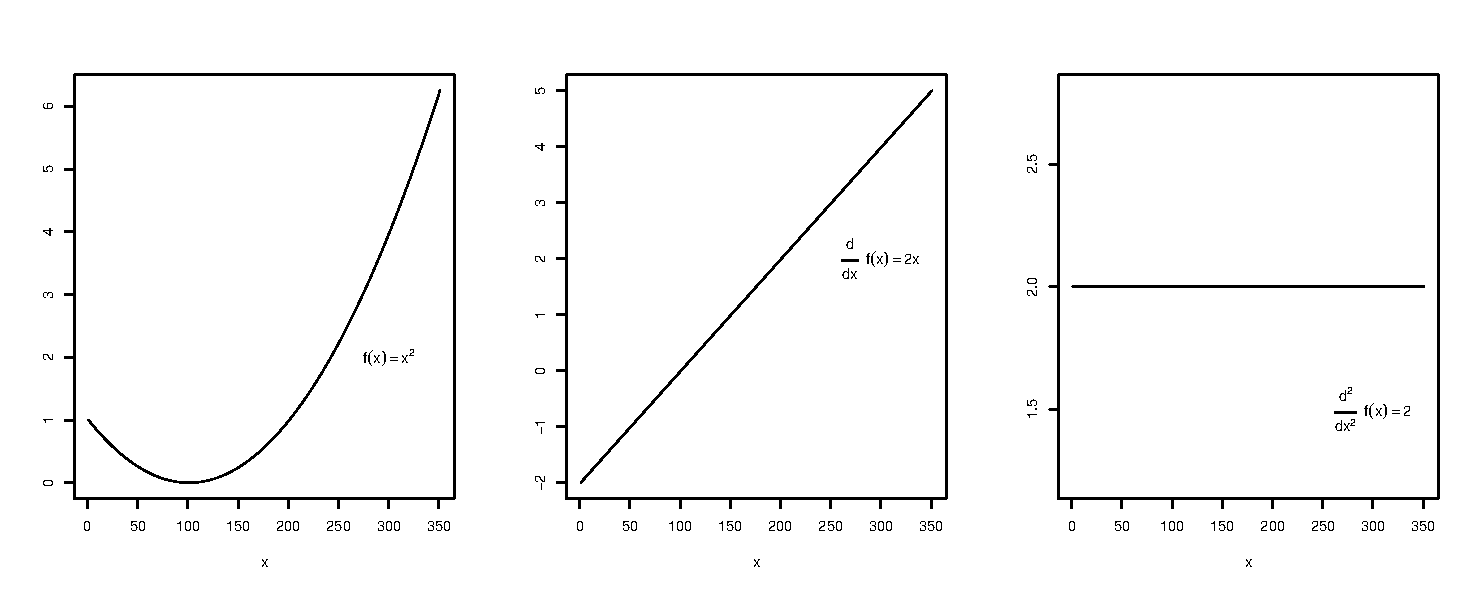
\includegraphics[width=6.5cm]{abb1.png}  % width legt Breite der Graphik fest

\begin{minipage}{0.8\linewidth}
\footnotesize{die Graphik sollte beschrieben werden, sodass man ohne den Text vorne zu lesen wei\ss{}, worum es geht: panel 1 zeigt die Funktion, panel 2 die erste Ableitung und Panel 3 die zweite Ableitung}
\end{minipage}

\end{figure}

\begin{figure}
\caption{titel der Graphik}
\label{fig:andereGraphik} \centering
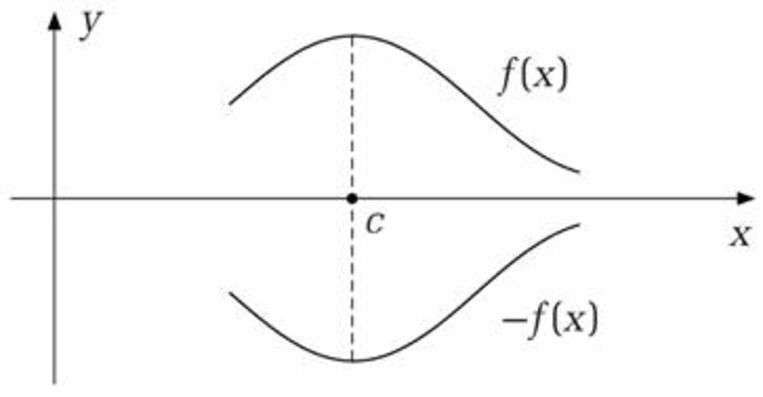
\includegraphics[angle=90,height=6.5cm]{abb2.jpg}  % angle dreht die Graphik, falls noetig; height legt die Hoehe der Graphik fest

\end{figure}

\begin{table}
\caption{Der Title der Tabelle}
\label{tab:Tabelle}
\centering
 \begin{tabular}{lc|r}
   Eine & kleine & Tabelle\\
\hline
   Text links & mittig & oder rechts \\
   & unterstrichen  & \\
\cline{2-2}
   \multicolumn{2}{c|}{\"uber zwei Spalten} & dritte Spalte \\
\end{tabular}   
\end{table}

   





\end{document}
